\chapter{Results and Discussion}
\label{chap:result}

After the like-sign background removal, the raw spectra are then corrected for the detector efficiency losses. The invariant mass, transverse momentum, and centrality differential measurements of dielectron yields within STAR acceptance, compared to Monte-Carlo hadronic contributions (excluding $\rho$-meson) and model calculations, are reported in this chapter. In particular, the dielectron production at very low $p_{T}$ ($p_{T}$ < 0.15 GeV/$c$) in peripheral collisions which may have a link to the photoproduction, are also discussed. Furthermore, the detector acceptance corrections for the excess spectra (dielectron invariant mass spectrum with hadronic contributions except $\rho$-meson removed) are applied. System-size and energy dependences of low mass excess yield are reported together with model comparisons.

\section{Dielectron Invariant Mass Spectra in Minimum-Bias Collisions}
\label{broadenedrho}
The dielectron invariant mass spectrum measured within STAR acceptance ( $p_{T}^{e}$ > 0.2 GeV/$c$, $|\eta^{e}|$ < 1 and $|y_{ee}|$ < 1) in U + U minimum-bias collisions (0 - 80\%) at $\sqrt{s_{NN}}$ = 193 GeV is shown in the top panel of Fig.~\ref{minibias_spec}. The vertical bars represent the statistical errors while the gray boxes represent the systematic uncertainties of the data. The data are compared with the hadronic cocktail simulation without the $\rho$ meson contribution. The $\rho$ meson is expected to be modified by the hot, dense medium created in U + U collisions, thus the contribution of $\rho$ mesons is left for theoretical input which will be discussed later. The data over hadronic cocktail ratio as a function of invariant mass is shown in the bottom panel of Fig.~\ref{minibias_spec}. The yellow band is the systematic uncertainty of the cocktail simulation. A significant enhancement of dielectron yields is observed with respect to the hadronic cocktail simulation without $\rho$ contribution in the LMR. The data, integrated in the $\rho$-like mass region (0.30 < $M_{ee}$ < 0.76 GeV/$c^{2}$), is a factor of 2.11 $\pm$ 0.11(stat.) $\pm$ 0.23(sys.) $\pm$ 0.27(cocktail) larger than the cocktail simulation. In the IMR, the cocktail is dominated by the charm contribution, and the measured dielectron yields are consistent with the cocktail simulation. However, no conclusive evidence for contributions from other sources (e.g. QGP thermal radiation) can be ruled out due to the limits of the data precision and our present understanding of the modification of the charmed hadron production in heavy-ion collisions.
 
\begin{figure}[htbp]
\centering
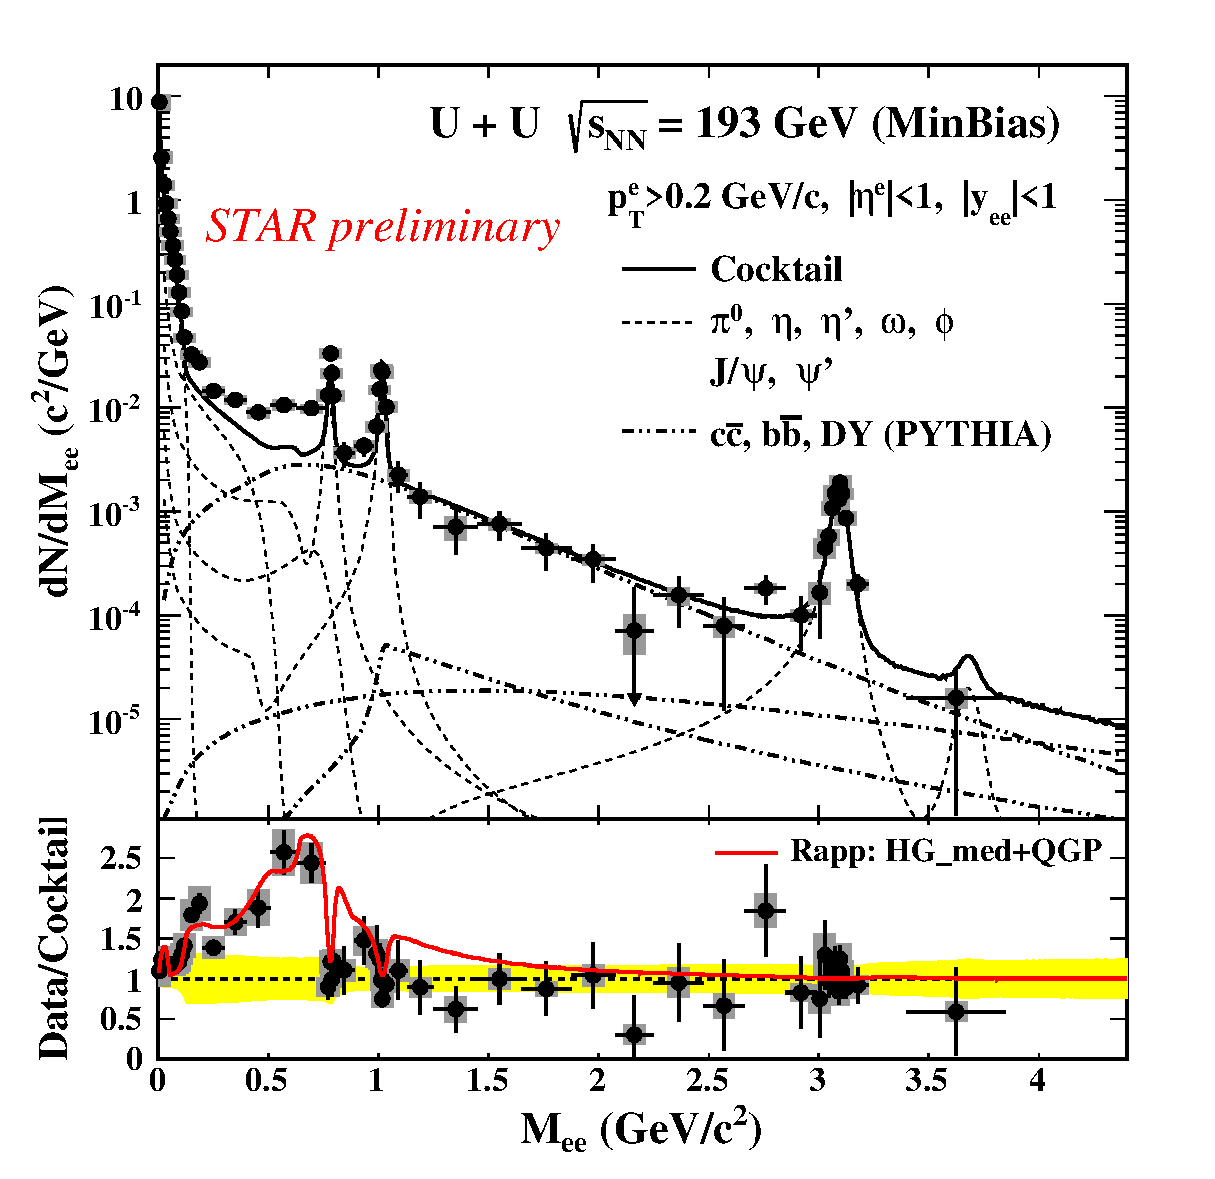
\includegraphics[keepaspectratio,width=0.8\textwidth]{results/minibias_dielectronSpec.eps}
\figcaption{(Top) Dielectron invariant mass spectrum within STAR acceptance ($p_{T}^{e}$> 0.2 GeV/$c$, $|\eta^{e}|<$ 1, and $|y_{ee}|<$ 1) in U + U minimum-bias collisions at $\sqrt{s_{NN}}$ = 193 GeV, compared with hadronic cocktail simulation (solid line) including light hadron decays and correlated heavy flavor decays (dashed lines).  (Bottom) The ratio of dielectron yield over cocktail with a theoretical model~\cite{broaden1,broaden2,broaden3,broaden4} comparison. Gray boxes represent the systematic uncertainties of the data. Yellow bands depict systematic uncertainties of the cocktail simulation.}
 \label{minibias_spec}
\end{figure}

As mentioned in the Sec.~\ref{dilepton:physics}, theoretical calculations suggest that the vector meson spectral functions will undergo modifications in a hot and dense hadronic medium, which are considered as a link to chiral symmetry restoration. There are two chiral symmetry restoration scenarios commonly used in calculations: (a) the drop of pole mass~\cite{dropmass} and the broadening of the spectral function~\cite{broaden0,broaden1,broaden2,broaden3,broaden4}. The precise measurements from the NA60 experiment at $\sqrt{s_{NN}}$ = 17.3 GeV demonstrated that an in-medium broadened $\rho$ scenario could reproduce the low mass dilepton enhancement, while the dropping mass scenario failed to describe this enhancement~\cite{NA60:dimuon0,NA60:dimuon3}. With the total baryon density nearly a constant and the dilepton emission rate dominant in the critical temperature from top RHIC energy down to the top SPS energy, the characteristic of dilepton production in the LMR region is expected to be similar between RHIC and SPS. However, the QGP contribution is expected to become sizable for $M_{ll}$ > 1.5 GeV/$c^{2}$ at top RHIC energy owing to a well-established partonic phase~\cite{broaden1}.

A model calculation (``macroscopic effective many-body theory model'') containing a broadened $\rho$ spectral function (HG\_med) and QGP thermal radiation from Rapp $et\,al.$~\cite{broaden1,broaden2,broaden3,broaden4} is added to the hadronic cocktail and compared with the data. The comparison shows the model calculation is consistent with the data within uncertainties, as shown in the bottom panel of Fig.~\ref{minibias_spec}. The model calculation involves a realistic space-time evolution, and the dielectron yields in the model calculation are integrated over the full space-time evolution and filtered by STAR acceptance. In this model, the dilepton production in the hadronic medium is calculated via electromagnetic correlators based on the vector-meson dominance model (VDM) approach trough a macroscopic (thermal) medium evolution. The $\rho$-meson propagator is calculated from the interactions of the $\rho$ with mesons and baryons. The dilepton yields are determined by the $\rho$ propagator in the medium with an assumption of a thermal equilibrated hadronic medium. Many theoretical calculations~\cite{dileptonMed0,dileptonMed1,dileptonMed2} show that the coupling with baryons in the medium plays a dominate role in the broadening of the $\rho$ spectral function. Thus, the medium total baryon density is a critical factor in determining the dielectron yield in heavy-ion collisions at these energies. The dilepton production in the partonic phase (QGP) is calculated via perturbative $q\bar{q}$ annihilation with nonperturbative corrections inferred from lattice QCD. The theoretical calculation has demonstrated that the dilepton emission rates from the hadronic medium should be equivalent to the rates from the partonic phase, dominant in the critical temperature ($T_{c}$) region, which is known as ``parton-hadron'' duality~\cite{LMRDileptonTheory}.

\section{$p_{T}$ Dependence of The Dielectron Spectra}
The differential measurements of dielectron spectra within STAR acceptance in various $p_{T}$ bins, together with the corresponding hadronic cocktails, are shown in the left panel of Fig.~\ref{diffpt_spectra}. The corresponding ratios of data over cocktail simulations are shown in the right panel of Fig.~\ref{diffpt_spectra}. Enhancements in the LMR are consistently observed compared with corresponding hardronic cocktails in all $p_{T}$ bins.  These enhancements can be consistently described by the broadened $\rho$ model calculation discussed in last section. To quantitatively describe the enhancements, the ratios of data over cocktail simulations and integrated dielectron yields in the $\rho$-like mass region (0.30 $<M_{ee}<$ 0.76 GeV/$c^{2}$) are calculated and summarized in Tab.~\ref{diffpt_yields}. The relative enhancement in the data compared to the cocktail has no obvious $p_{T}$ dependence.

\begin{figure}[htbp]
\centering
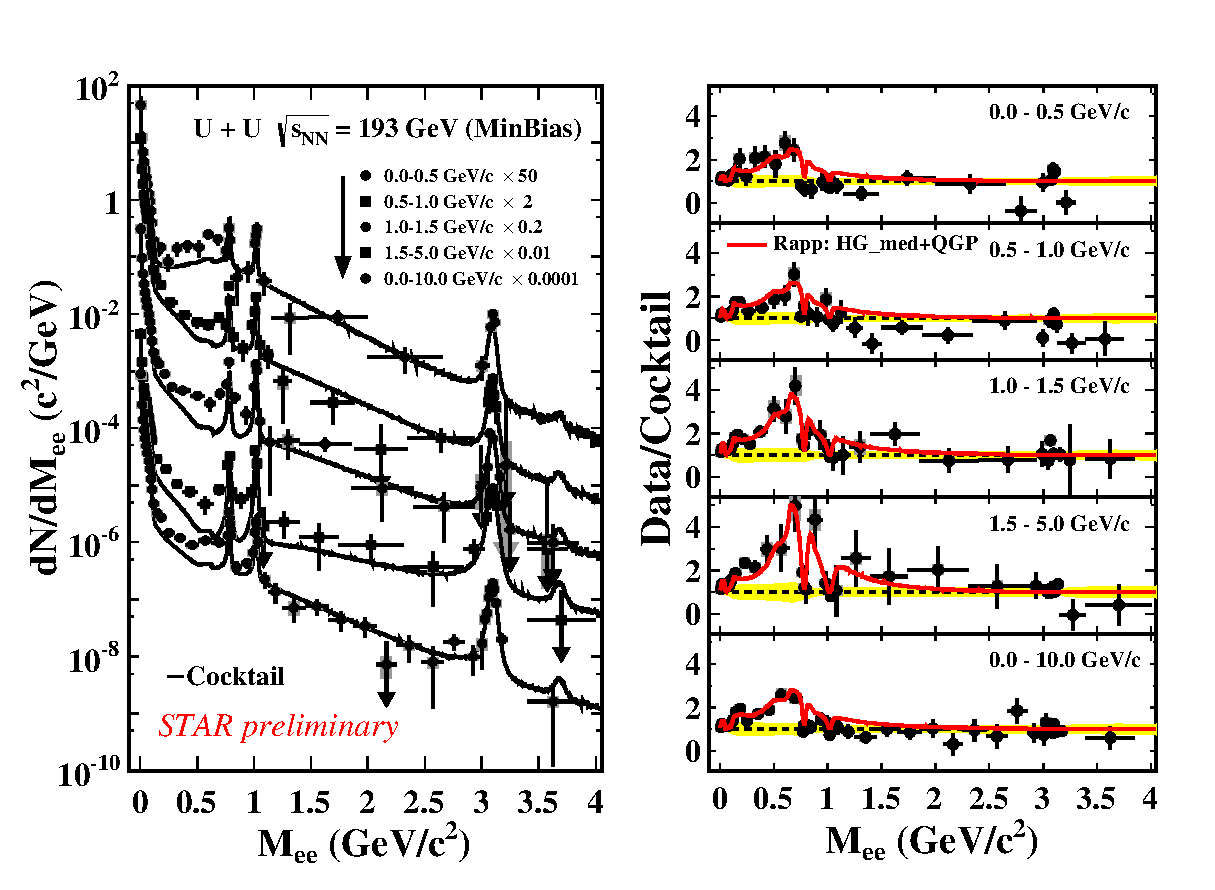
\includegraphics[keepaspectratio,width=0.8\textwidth]{results/diffPtBins_dielectronSpec.eps}
\figcaption{(Left) Invariant mass spectra from $\sqrt{s_{NN}}$ = 193 GeV U + U minimum-bias collisions in different $p_{T}$ bins. The solid curves represent the hadronic cocktail simulations. (Right) The ratios of dielectron yield over cocktail for different $p_{T}$ bins with theoretical model comparisons. Gray boxes (arrows) show the systematic uncertainties of the data. Yellow bands depict systematic uncertainties of the cocktail simulations.}
 \label{diffpt_spectra}
\end{figure}

\begin{figure}[htbp]
\centering
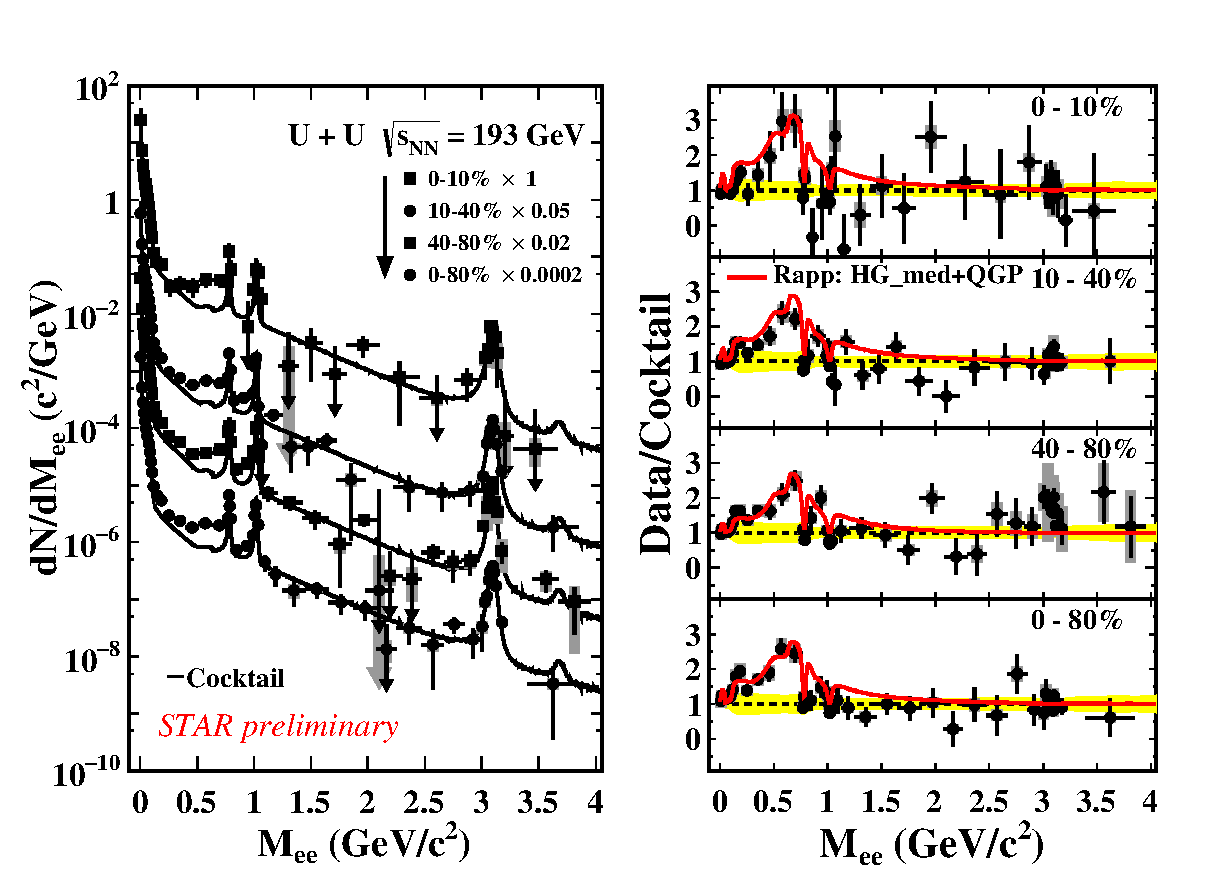
\includegraphics[keepaspectratio,width=0.8\textwidth]{results/diffCenBins_dielectronSpec.eps}
\figcaption{ (Left) Invariant mass spectra from $\sqrt{s_{NN}}$ = 193 GeV U + U collisions in different centralities. The solid curves represent the hadronic cocktail simulations. (Right) The ratios of dielectron yield over cocktail for different centralities with theoretical model comparisons. Gray boxes (arrows) show the systematic uncertainties of the data. Yellow bands depict systematic uncertainties of the cocktail simulations.}
 \label{diffcen_spectra}
\end{figure}

\section{Centrality Dependence of The Dielectron Spectra and Low-Mass Excess Yields}
The dielectron spectra within STAR acceptance are also studied in various centrality bins (0-10\%, 10-40\%, and 40-80\%). The dielectron spectra together with the hadronic cocktails are shown in the left panel of Fig.~\ref{diffcen_spectra} while the ratios of data over cocktail are shown in the right panels. The same broadened $\rho$ model calculations are added to the ratio plots for comparison.  The ratios of data over cocktail simulations and integrated dielectron yields in the $\rho$-like mass region (0.30 $<M_{ee}<$ 0.76 GeV/$c^{2}$) are summarized in Tab.~\ref{diffcen_yields}. The enhancement factor with respect to the cocktail (data/cocktail) in the $\rho$-like mass region does not show a significant centrality dependence within the uncertainty. The correlated charm contributions, which become very important in the mass region in the mass region 0.50 $<M_{ee}<$ 3.0 GeV/$c^{2}$, are all taken from the PYTHIA simulation (discussed in Sec.~\ref{cocktail}) and then scaled by $N_{coll}$.

\begin{table}[htp]
\centering
\caption{The $p_{T}$ dependence of the integrated yields and enhancement factor with respect to cocktail within STAR acceptance in the $\rho$-like mass region (0.30 $<M_{ee}<$ 0.76 GeV/$c^{2}$).}
\label{diffpt_yields}
\newcolumntype{V}{!{\vrule width 1.6pt}}
\begin{tabular}{ccc}
\Xhline{1.6pt}
 $p_{T}$ (GeV/$c$) &  Yield ($\times10^{-3}$) & Yield/Cocktail \\
\Xhline{1.2pt}
0-0.5    & 1.55 $\pm$ 0.17 $\pm$ 0.39 & 2.16 $\pm$ 0.24 $\pm$ 0.54 \\ 
0.5-1.0 & 1.69 $\pm$ 0.15 $\pm$ 0.31 & 1.82 $\pm$ 0.16 $\pm$ 0.33 \\ 
1.0-1.5 & 0.83 $\pm$ 0.08 $\pm$ 0.16 & 2.68 $\pm$ 0.25 $\pm$ 0.50 \\ 
1.5-5.0 & 0.31 $\pm$ 0.04 $\pm$ 0.07 & 3.12 $\pm$ 0.39 $\pm$ 0.75 \\ 
\Xhline{1.6pt}
\end{tabular}
\end{table}

\begin{table}[htp]
\centering
\caption{The centrality dependence of the integrated yields and enhancement factor with respect to cocktail within STAR acceptance in the $\rho$-like mass region (0.30 $<M_{ee}<$ 0.76 GeV/$c^{2}$).}
\label{diffcen_yields}
\newcolumntype{V}{!{\vrule width 1.6pt}}
\begin{tabular}{ccc}
\Xhline{1.6pt}
 Centrality (\%) &  Yield ($\times10^{-3}$) & Yield/Cocktail \\
\Xhline{1.2pt}
0-10   & 16.49 $\pm$ 2.47 $\pm$ 1.84 & 2.23 $\pm$ 0.33 $\pm$ 0.25 \\ 
10-40 &   5.97 $\pm$ 0.41 $\pm$ 0.68 & 1.88 $\pm$ 0.13 $\pm$ 0.22 \\ 
40-80 &   0.98 $\pm$ 0.06 $\pm$ 0.10 & 1.90 $\pm$ 0.12 $\pm$ 0.20 \\ 
0-80   &   4.74 $\pm$ 0.26 $\pm$ 0.51 & 2.11 $\pm$ 0.11 $\pm$ 0.23 \\ 
\Xhline{1.6pt}
\end{tabular}
\end{table}

Figure~\ref{diffcen_excess_spectra} shows the dielectron excess invariant mass spectra (data - cocktail) within STAR acceptance in the mass region 0.3 $< M_{ee} <$ 1.25 GeV/$c^{2}$ for 40-80\%, 10-40\%, and 0-10\% U + U collisons at $\sqrt{s_{NN}}$ = 193 GeV. From Fig.~\ref{diffcen_spectra} (right panels) and Fig.~\ref{diffcen_excess_spectra}, we can see that the broadened $\rho$ model calculation can well describe the LMR region enhancements for all centrality bins. The dielectron mass integral excess yields within STAR acceptance in the $\rho$-like mass region scaled by $N_{part}$ (number of participants) as a function of $N_{part}$ are shown in Fig.~\ref{diffcen_excess_yield}. The integral excess yields in U + U collisons at $\sqrt{s_{NN}}$ = 193 GeV, following a similar trend in Au + Au collisons at $\sqrt{s_{NN}}$ = 200 GeV~\cite{STAR:dielectron1}, increase faster than $N_{part}$ scaling as a function of centrality, indicating that the dielectron yields in the $\rho$-like region are sensitive to the QCD medium dynamics, as expected by the theoretical calculations~\cite{rhopeak,broaden4}.
 
\begin{figure}[htbp]
\begin{minipage}[htbp]{0.50\linewidth}
\centering
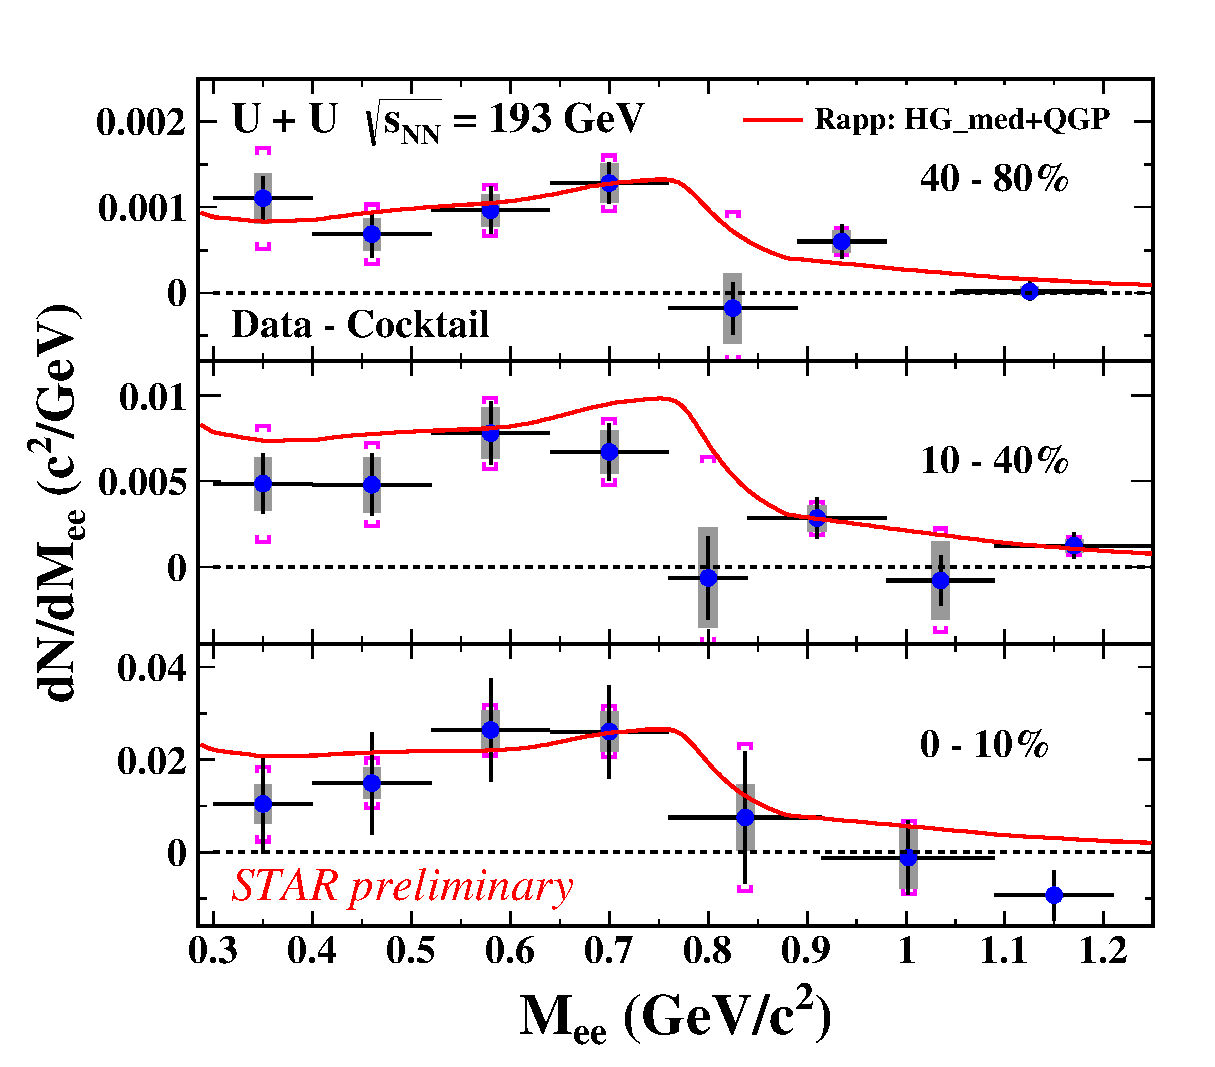
\includegraphics[width=0.9\textwidth]{results/diffCenBins_excessSpec.eps}
\caption{Mass spectra of the excess (data - cocktail) within STAR acceptance in the LMR for 40-80\%, 10-40\%, and 0-10\% U + U collisions at $\sqrt{s_{NN}}$ = 193 GeV, compared with a model calculation (red lines). Gray boxes represent the systematic uncertainties for the data. Magenta brackets depict the total systematic uncertainties including those from cocktails. \label{diffcen_excess_spectra}}
\end{minipage}
\hfill
\begin{minipage}[htbp]{0.48\linewidth}
\centering
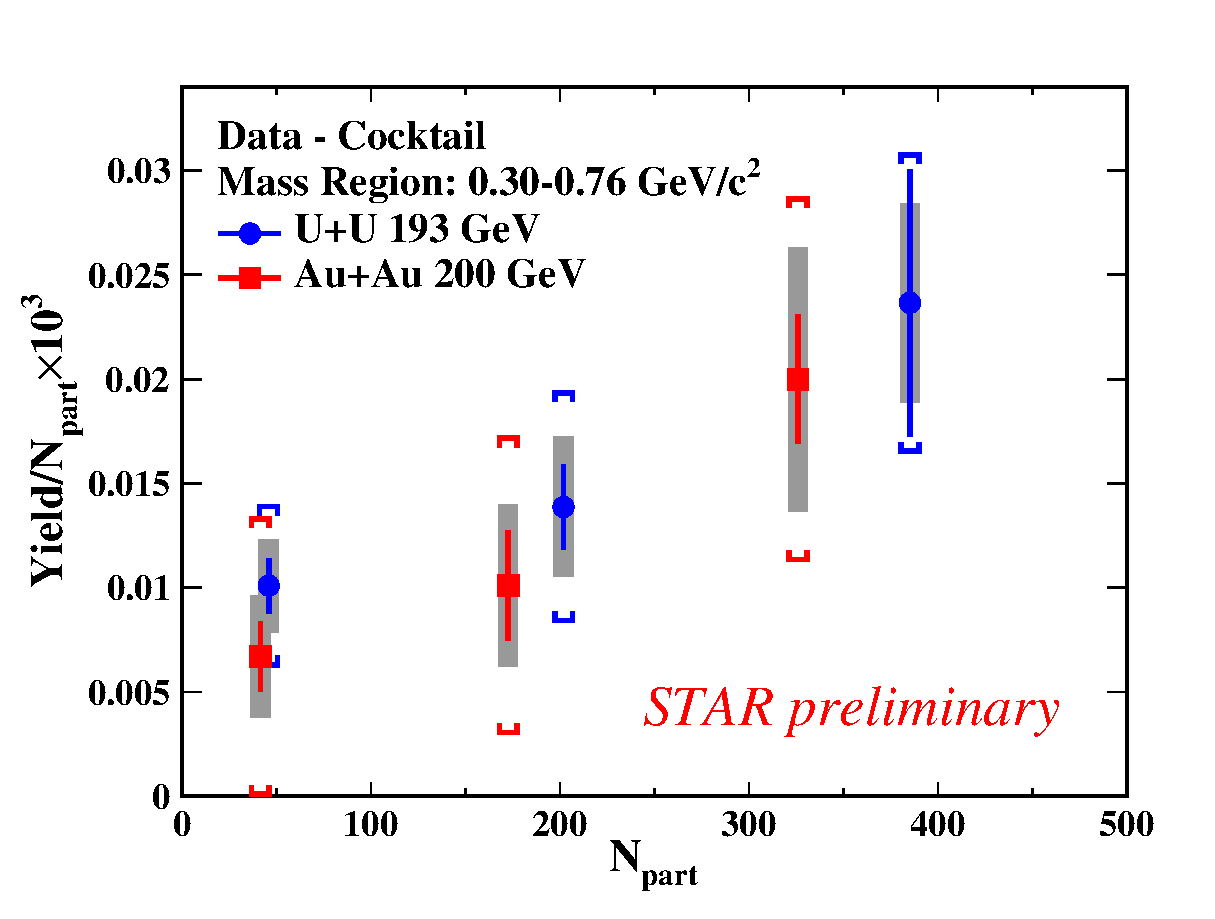
\includegraphics[width=1.0\textwidth]{results/diffCenBins_yield.eps} 
\caption{The dielectron excess yield within STAR acceptance scaled by $N_{part}$ in the $\rho$-like mass region as a function of  $N_{part}$. The blue solid circles are the results for 40-80\%, 10-40\%, and 0-10\% U + U collisions at $\sqrt{s_{NN}}$ = 193 GeV. The red solid squares are the results for 40-80\%, 10-40\%, and 0-10\% Au + Au collisions at $\sqrt{s_{NN}}$ = 200 GeV~\cite{STAR:dielectron1}. Gray boxes represent the systematic uncertainties of the data. Red and blue brackets depict the total systematic uncertainties including those from cocktails.\label{diffcen_excess_yield}}
\end{minipage}
\end{figure}

\section{STAR Acceptance-corrected Dielectron Spectrum and Excess Yields}
To quantify the excess yields and quantitatively study the medium properties, the excess spectra are needed to be corrected for the detector acceptance. The acceptance correction is evaluated by a Toy Monte Carlo simulation using virtual photon as input (see details in Sec.~\ref{paireff}), and the 2-D acceptance correction factor for U + U minimum-bias collisions at 193 GeV can be found in the left panel of Fig.~\ref{acceptance2d}. The STAR acceptance-corrected excess spectrum for U + U minimum-bias collisions at 193 GeV is shown in Fig.~\ref{acc_excess_spec}. The spectrum are normalized by charged particle density at mid-rapidity ($dN_{ch}/dy$) to cancel out the volume effect, and compared with the same broadened $\rho$ model calculation from Rapp $et\,al.$~\cite{broaden1,broaden3,broaden4}. The model calculation is consistent with the acceptance-corrected excess invariant mass spectra within uncertainty. To quantitatively compare the excess in the LMR, the $dN_{ch}/dy$ normalized integral yields of excess invariant mass spectra in the mass region 0.4 $<M_{ll}<$ 0.75 GeV/$c^{2}$ for different collision species and collision energies as a function of $dN_{ch}/dy$ are shown in Fig.~\ref{intExcessYield}. The lifetime given by the same model calculations, which consistently describe the dielectron excess of SPS and RHIC data~\cite{CERES:dielectron3,NA60:dimuon0,PHENIX:dielectron1,STAR:dielectron1}, are also shown as dashed lines and horizontal bars in Fig.~\ref{intExcessYield}. We can clearly see the theoretical medium lifetime has collision energy dependence and strong centrality dependence in U + U collisions at 193 GeV and Au + Au collisions at 200 GeV. The normalized integral excess yields have a centrality dependence and increase from peripheral to central collisions in U + U collisions at $\sqrt{s_{NN}}$ = 193 GeV and Au + Au collisions at $\sqrt{s_{NN}}$ = 200 GeV. Moreover, the normalized integral yields of the most central U + U collisions at $\sqrt{s_{NN}}$ = 193 GeV and Au + Au collisions at $\sqrt{s_{NN}}$ = 200 GeV are higher than those at lower energies. With total baryon density nearly a constant (as shown in Fig.~\ref{ppiratio}) and the dilepton emission rate dominant in the critical temperature region ($T_{c}$) at $\sqrt{s_{NN}}$ = 17.3 - 200 GeV, the normalized integral excess yields in LMR is proportional to the medium lifetime~\cite{lifetime_cal}. Those measurements indicate that the hot and dense medium created in central U + U collisions at $\sqrt{s_{NN}}$ = 193 GeV and Au + Au collisions at $\sqrt{s_{NN}}$ = 200 GeV has longer lifetime than those in peripheral or low-energy collisions, which enhances the dilepton production from thermal radiation.

\begin{figure}[htbp]
\centering
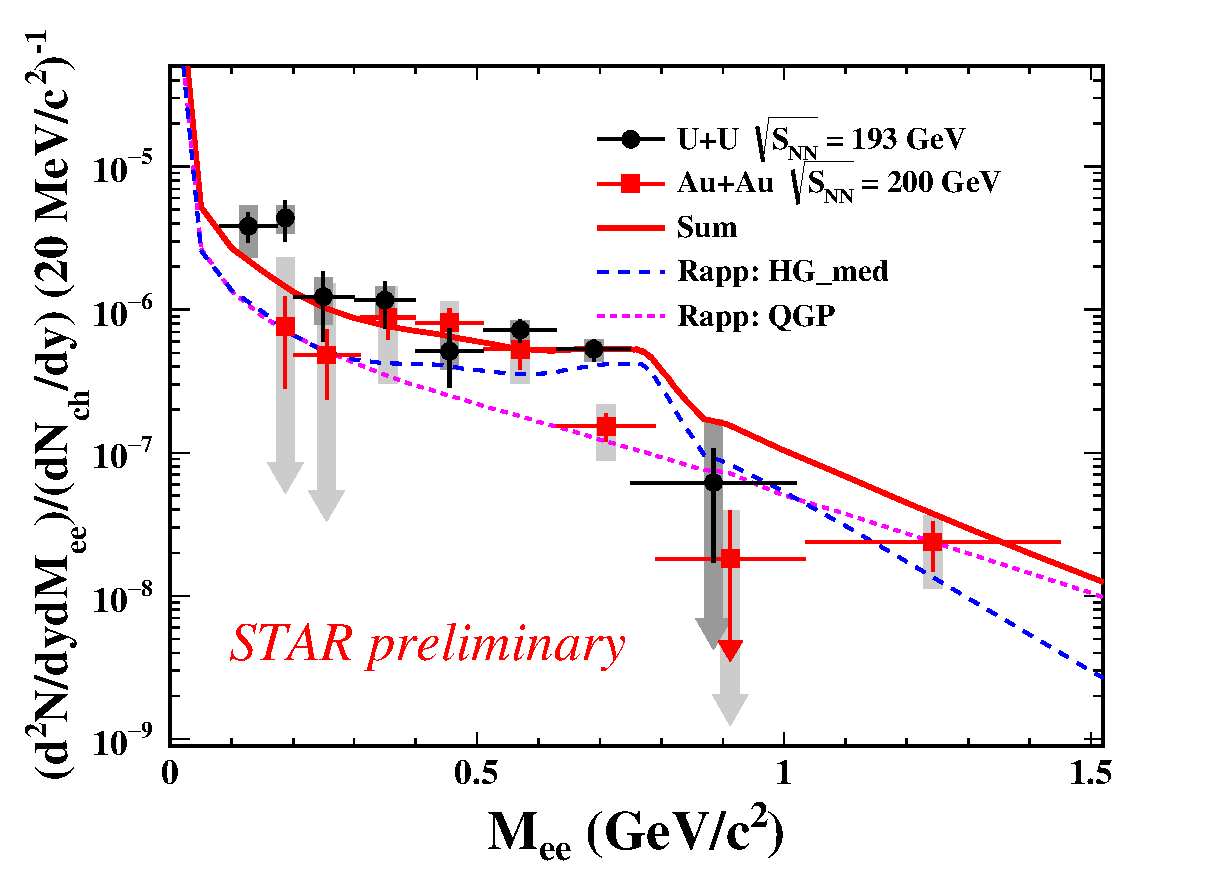
\includegraphics[keepaspectratio,width=0.8\textwidth]{results/Excess_The_193.eps}
\figcaption{STAR acceptance-corrected dielectron excess invariant mass spectra, normalized by $dN_{ch}/dy$, in minimum-bias U + U collisions at 193 GeV (red squares) and Au + Au collisions at 200 GeV (black dots). A model calculation for Au + Au collisions at 200 GeV (red solid curve)~\cite{broaden1,broaden2,broaden3,broaden4} containing a broadened $\rho$ spectral function in hadronic medium (blue dashed curve) and QGP thermal radiation (magenta dashed curve) is compared with data.}
 \label{acc_excess_spec}
\end{figure}

\begin{figure}[htbp]
\centering
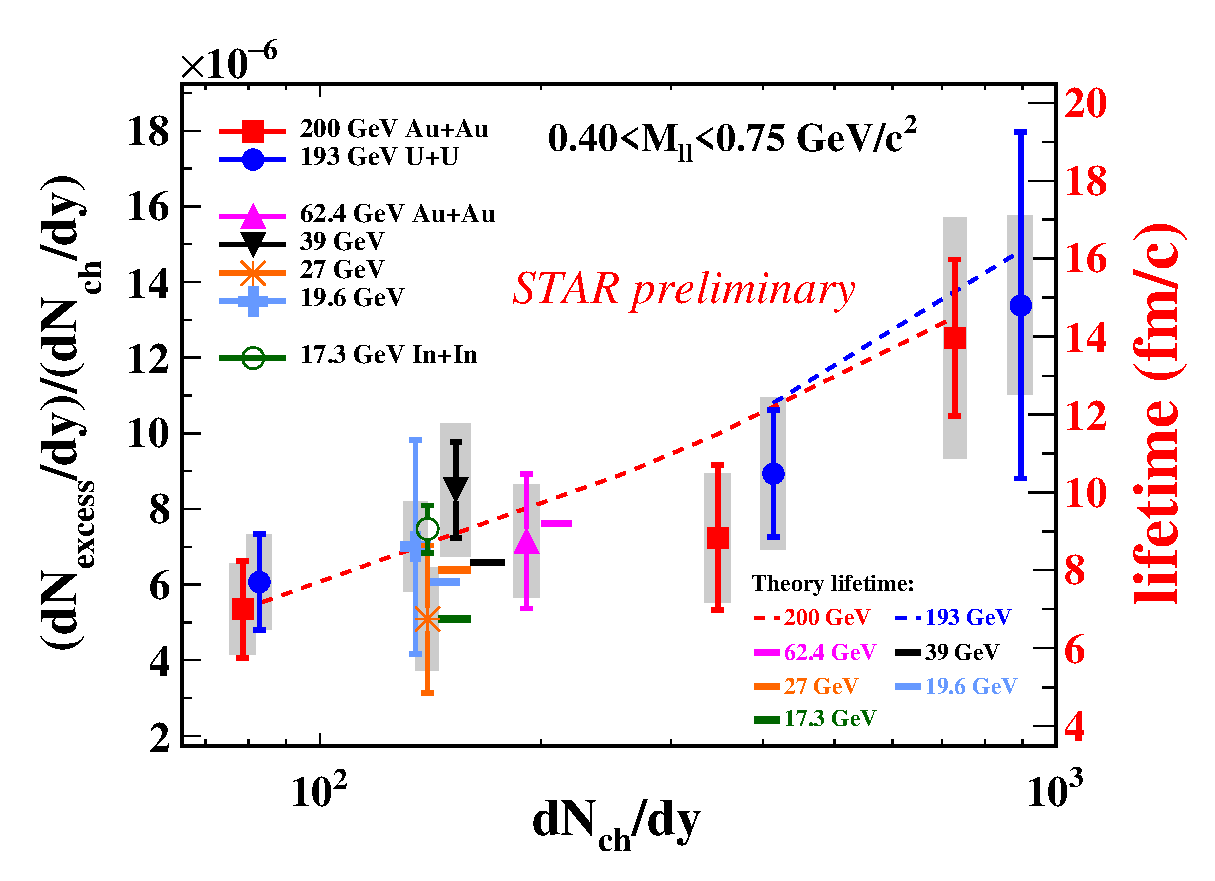
\includegraphics[keepaspectratio,width=0.8\textwidth]{results/IntExcess.eps}
\figcaption{The $dN_{ch}/dy$ normalized integral yields of  dilepton excess invariant mass spectra in different collision species and collision energies for 0.40 $<$ $M_{ll}$ $<$ 0.75 GeV/$c^{2}$ as a function of $dN_{ch}/dy$ (In + In@17.3 GeV~\cite{NA60:dimuon4}, Au + Au@19.6, 200 GeV~\cite{STAR:dielectron2}, Au + Au@27, 39, 62 GeV~\cite{dielectoninUU193}). The blue solid circles are the results for 40-80\%, 10-40\%, and 0-10\% U + U collisions at $\sqrt{s_{NN}}$ = 193 GeV. The red solid squares are the results for 40-80\%, 10-40\%, and 0-10\% Au + Au collisions at $\sqrt{s_{NN}}$ = 200 GeV. The theoretical lifetime inputs in the model calculations~\cite{lifetime_cal} are shown as dash lines and horizontal bars are shown as dash lines and horizontal bars.}
 \label{intExcessYield}
\end{figure}

\section{Low $p_{T}$ Dielectron Production in U + U Peripheral Collisions}
The photoproduction $\rho^{0}$, $J/\psi$ and $\psi$(2$S$) in the ultra-peripheral heavy-ion collisions have been reported by STAR, PHENIX and ALICE collaborations~\cite{STARUPCrho0,STARUPCrho1,PHENIXUPCjpsi,ALICEUPCjpsi}. These results are consistent with the theoretical models for the coherent photoproduction. Recently, an excess $J/\psi$ yield at very low transverse momentum ($p_{T}$ < 0.3 GeV/$c$) in peripheral Pb + Pb collisions has been reported by ALICE~\cite{ALICEPCjpsi}. The observed excess is interpreted with coherent photoproduction of $J/\psi$ at the moment. If the $\rho$ meson can be produced via coherent photoproduction process in the peripheral heavy-ion collisions, it might sit in QGP. This will provide a direct probe of the QGP. In the following two sub-sections, the low $p_{T}$ dielectron productions in U + U peripheral collisions at $\sqrt{s_{NN}}$ = 193 GeV are discussed.

\subsection{The $p_{T}$ Dependence of Dielectron Mass Spectra for Different Centralities.}
The U + U minimum-bias data sample is divided into four centrality classes (0-10\%, 10-40\%, 40-60\%, and 60-80\%) according to the uncorrected charge particle density (discussed in Sec.~\ref{centrality}). For each centrality class, the dielectron mass spectra within STAR acceptance are studied in there $p_{T}$ bins (0-0.15 GeV/$c$, 0.15-0.30 GeV/$c$, and 0.30-10.0 GeV/$c$). Figure~\ref{lowptMassSpec_Cen60_80} shows the efficiency-corrected mass spectrum within STAR acceptance at very low $p_{T}$ ($p_{T}$ < 0.15 GeV/$c$) in peripheral U + U collisions (60-80\%), where a significant enhancement with respect to hadronic cocktail simulation (without $\rho$ contribution) can be observed for the entire mass region. The $p_{T}$ distributions of hadrons used in cocktail simulation at very low $p_{T}$ are extrapolated from the measurements at higher $p_{T}$. The integrated yield in 0.40 $<M_{ee}<$ 0.76 GeV/$c^{2}$, is a factor of 16.4 $\pm$ 1.1(stat.) $\pm$ 2.6(sys.) $\pm$ 4.2(cocktail) larger than the cocktail simulation. While the relative enhancement factor in 2.8 $<M_{ee}<$ 3.2 GeV/$c^{2}$ ($J/\psi$ mass region) is 20.4 $\pm$ 4.2(stat.) $\pm$ 3.0(sys.) $\pm$ 3.2(cocktail). Figure~\ref{lowptExcessSpec_Cen60_80} depicts the corresponding excess spectrum (data-cocktail) together with the same broadened $\rho$ model calculation discussed in Sec.~\ref{broadenedrho}. The broadened $\rho$ theoretical model calculation for the centrality 60-80\% is evaluated from that of minimum-bias (0-80\%) by $N_{part}$ scaling. We can clearly see that the broadened $\rho$ model calculation can not account for the excess yields in the mass region 0.40 $<M_{ee}<$ 0.76 GeV$/c^{2}$. Thus, there are significant contributions from other sources, such as coherent photoproduction. The mass spectra in the $p_{T}$ region 0.15 $<p_{T}<$ 0.30 GeV/$c$ and 0.30 $<p_{T}<$ 10.0 GeV/$c$ in the same centrality class are shown in Fig.~\ref{highptMassSpec_Cen60_80}. An enhancement still can be observed, especially in the $J/\psi$ mass region, in 0.15 $<p_{T}<$ 0.30 GeV/$c$ though the statistics is limited. The enhancement factors in 0.40 $<M_{ee}<$ 0.76 GeV/$c^{2}$ and $J/\psi$ mass region in different $p_{T}$ regions in various centrality classes (except centrality 0-10\% bin due to the limited statistics) are listed in Tab.~\ref{enhancement:4diffpts}. These enhancement factors listed in Tab.~\ref{enhancement:4diffpts} reveal the enhancement mostly happens at very low $p_{T}$ in peripheral collisions.

\begin{figure}[htbp]
\begin{minipage}[htbp]{0.50\linewidth}
\centering
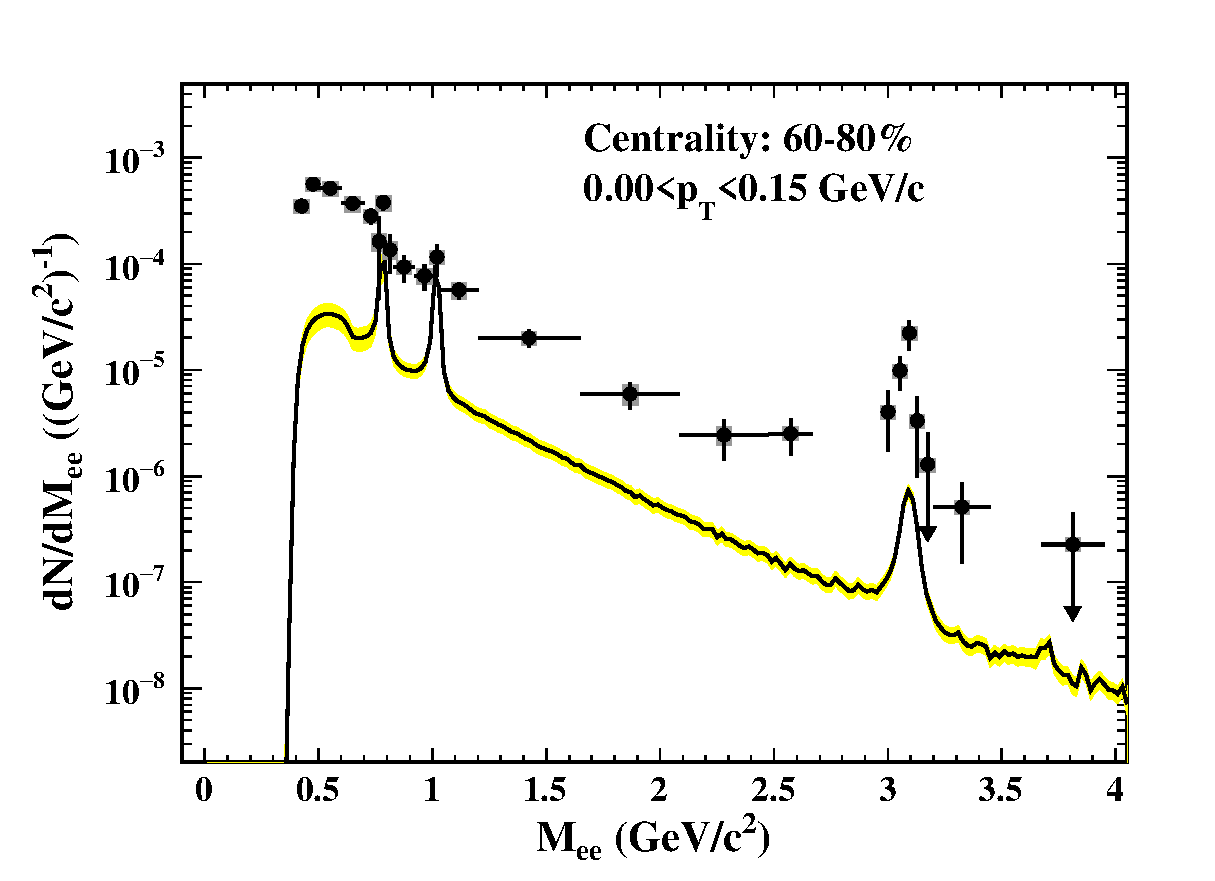
\includegraphics[width=0.9\textwidth]{results/diffPt_corrSignal_CenBin0_PtBin0.eps}
\caption{Dielectron invariant mass spectrum within STAR acceptance ($p_{T}^{e}$> 0.2 GeV/$c$, $|\eta^{e}|<$ 1, and $|y_{ee}|<$ 1) at very low $p_{T}$ ($ p_{T}<$ 0.15 GeV/$c$) in U + U peripheral collisions (60-80\%) at $\sqrt{s_{NN}}$ = 193 GeV, compared with hadronic cocktail simulation (black solid line). Gray boxes depict the systematic uncertainties of the data. Yellow bands depict systematic uncertainties of the cocktail simulations. \label{lowptMassSpec_Cen60_80}}
\end{minipage}
\hfill
\begin{minipage}[htbp]{0.48\linewidth}
\centering
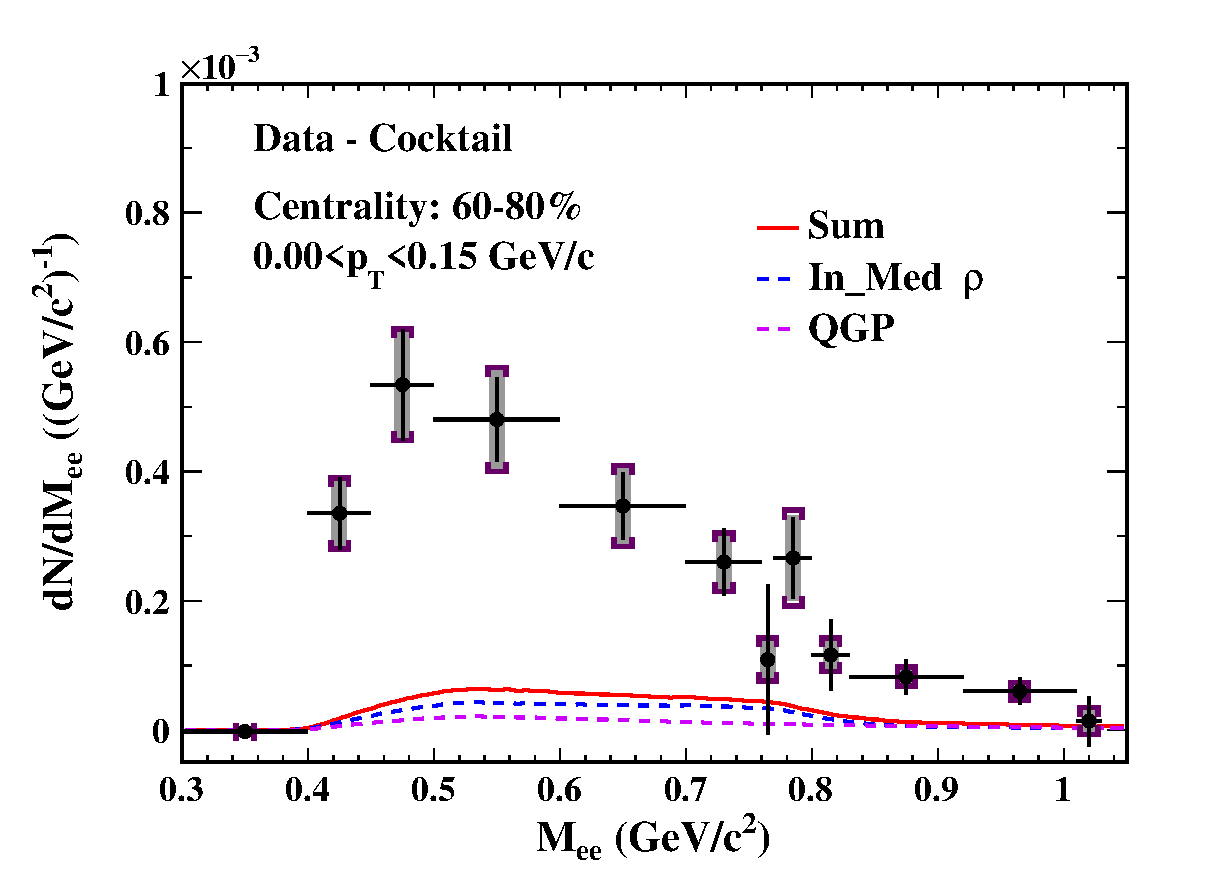
\includegraphics[width=1.0\textwidth]{results/diffPt_excessSpec_CenBin0_PtBin0.eps} 
\caption{Mass spectra of the excess (data - cocktail) within STAR acceptance in LMR at very low $p_{T}$ ($p_{T}<$ 0.15 GeV/$c$) in U + U peripheral collisions (60-80\%), together with a broadened $\rho$ model calculation (red solid line). Gray boxes represent the systematic uncertainties of the data. Dark violet brackets represent the total systematic uncertainties including those from cocktail simulation.\label{lowptExcessSpec_Cen60_80}}
\end{minipage}
\end{figure}

\begin{figure}[htbp]
\centering
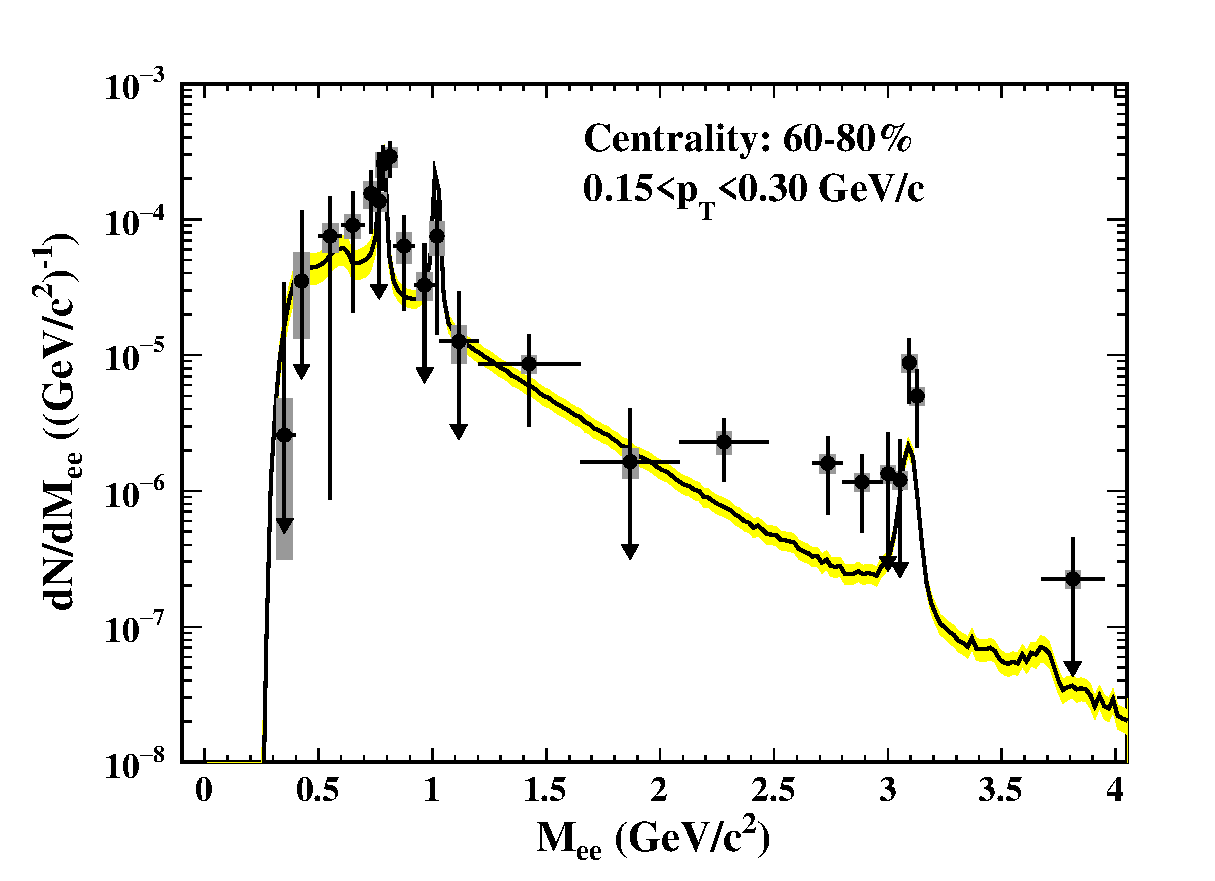
\includegraphics[width=0.49\textwidth]{results/diffPt_corrSignal_CenBin0_PtBin1.eps}
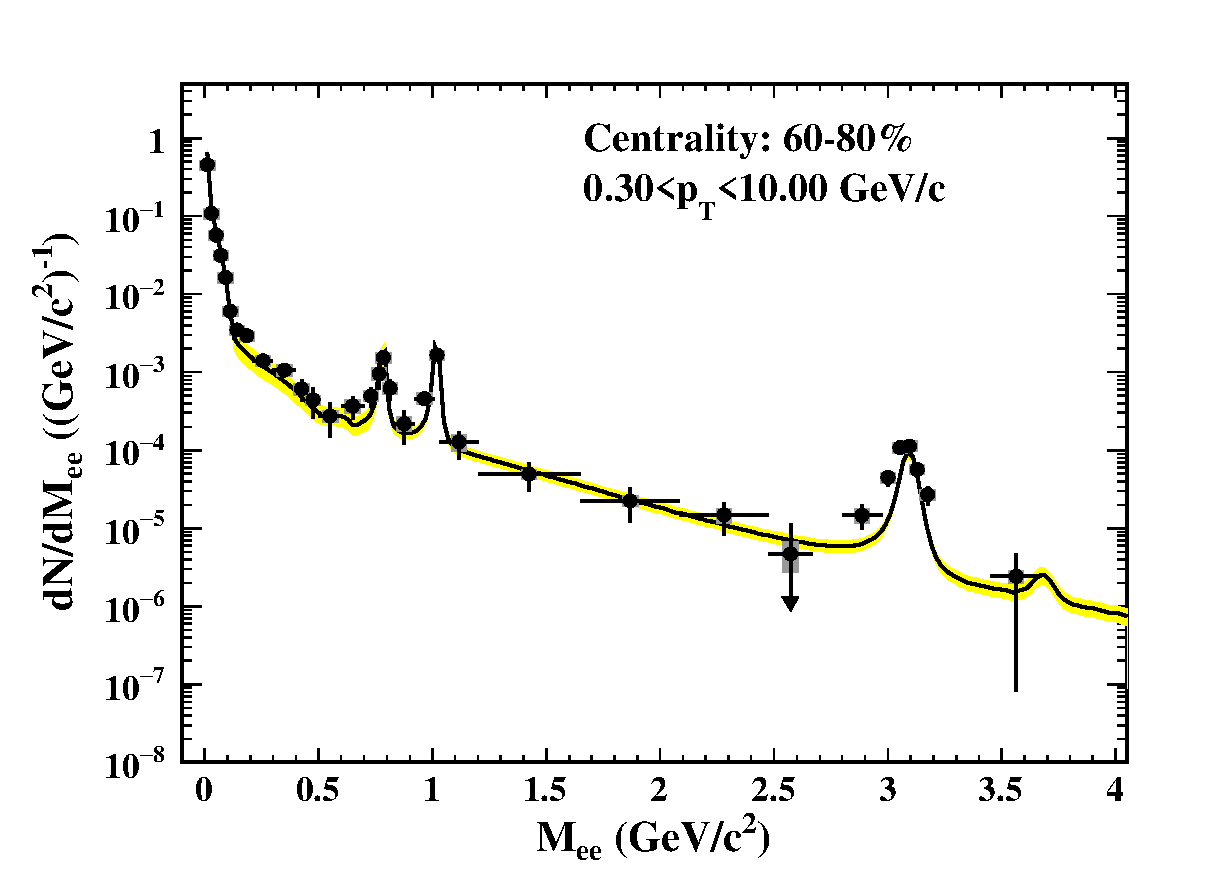
\includegraphics[width=0.49\textwidth]{results/diffPt_corrSignal_CenBin0_PtBin2.eps}
\figcaption{Dielectron invariant mass spectra within STAR acceptance in 0.15 $<p_{T}<$ 0.30 GeV/$c$ (Left) and 0.30 $<p_{T}<$ 10.0 GeV/$c$ (Right) in U + U peripheral collisions (60-80\%) at $\sqrt{s_{NN}}$ = 193 GeV, compared with hadronic cocktail simulations (black solid lines). Gray boxes depict the systematic uncertainties of the data. Yellow bands depict systematic uncertainties of the cocktail simulations.}
\label{highptMassSpec_Cen60_80}
\end{figure}

\begin{table}[htp]
\centering
\tabcaption{The $p_{T}$ dependence of the enhancement factor with respect to cocktail within STAR acceptance in 0.40 $< M_{ee} <$ 0.76 GeV/$c^{2}$ and  2.8 $< M_{ee} <$ 3.2 GeV/$c^{2}$ in various centrality bins.}
\label{enhancement:4diffpts}
\newcolumntype{V}{!{\vrule width 1.6pt}}
\begin{tabular}{cccc}
\Xhline{1.6pt}
\multirow{2}{*}{$p_{T}$ region (GeV/$c$)} & \multirow{2}{*}{Centrality (\%)} & \multirow{2}*{}{\thead{Yield/Cocktail \\ (0.4 $< M_{ee} <$ 0.76 GeV/$c^{2}$)}} &  \multirow{2}*{}{\thead{Yield/Cocktail \\ (2.8 $< M_{ee} <$ 3.2 GeV/$c^{2}$)}}\\
\Xhline{1.2pt}
\multirow{3}{*}{0 $<p_{T}<$ 0.15} & 60-80 & 16.4 $\pm$ 1.1 $\pm$ 2.6 & 20.4 $\pm$ 4.2 $\pm$ 3.0 \\
 & 40-60 & 5.4 $\pm$ 1.0 $\pm$ 1.0 & 7.8 $\pm$ 1.5 $\pm$ 1.4 \\
 & 10-40 & 3.1 $\pm$ 0.9 $\pm$ 0.6 & 2.8 $\pm$ 1.2 $\pm$ 0.7 \\
\Xhline{1.2pt}
\multirow{3}{*}{0.15 $<p_{T}<$ 0.3} & 60-80 & 1.4 $\pm$ 0.7 $\pm$ 0.4 & 3.5 $\pm$ 1.0 $\pm$ 0.5 \\
 & 40-60 & 1.2 $\pm$ 0.6 $\pm$ 0.3 & 1.2 $\pm$ 0.7 $\pm$ 0.3 \\
 & 10-40 & 1.1 $\pm$ 0.6 $\pm$ 0.4 & 2.8 $\pm$ 0.7 $\pm$ 0.6 \\
\Xhline{1.2pt}
\multirow{3}{*}{0.3 $<p_{T}<$ 10} & 60-80 & 1.3 $\pm$ 0.2 $\pm$ 0.2 & 1.8 $\pm$ 0.1 $\pm$ 0.3 \\
 & 40-60 & 1.7 $\pm$ 0.2 $\pm$ 0.3 & 1.2 $\pm$ 0.1 $\pm$ 0.2 \\
 & 10-40& 2.2 $\pm$ 0.2 $\pm$ 0.4 & 0.9 $\pm$ 0.1 $\pm$ 0.2 \\
\Xhline{1.6pt}
\end{tabular}
\end{table}

\subsection{The $p_{T}$ Spectra for Different Mass Regions in Different Centralities.}
To gain more insight into the dielectron enhancement at very low $p_{T}$ in the peripheral U + U collisions at $\sqrt{s_{NN}}$ = 193 GeV, the $p_{T}$ spectra in different mass regions (0.40 $<M_{ee}<$ 0.76 GeV/$c^{2}$, 1.20 $<M_{ee}<$ 2.67 GeV/$c^{2}$, 2.8 $<M_{ee}<$ 3.2 GeV/$c^{2}$) in various centrality classes (10-40\%, 40-60\%, and 60-80\%) are studied. The enhancement yields may be from different sources, such as $\gamma + Pomeron \rightarrow e^{+}e^{-}$ and $\gamma + \gamma \rightarrow e^{+}e^{-}$ processes~\cite{STARUPCrho0, PHENIXUPCjpsi}. The $p_{T}$ spectra of these two process may be different. Thus, it would be helpful to compare the $p_{T}$ spectra for different mass regions for understanding the enhanced signals. The efficiency-corrected $p_{T}$ spectra within STAR acceptance in different mass regions in different centrality classes are shown in Fig.~\ref{ptspec:4diffcens}. From the $p_{T}$ spectra, we can clearly observe significant enhancements in the low $p_{T}$ region (typically $p_{T}<$ 0.1 GeV/$c$) for all the three mass regions in the most peripheral (60-80\%) collisions, and the enhancements decrease toward central collisions. Moreover, the $p_{T}$ spectra in all the three mass regions have a fairly sharp transition around 0.1 GeV/$c$.

\begin{figure}[htbp]
\centering
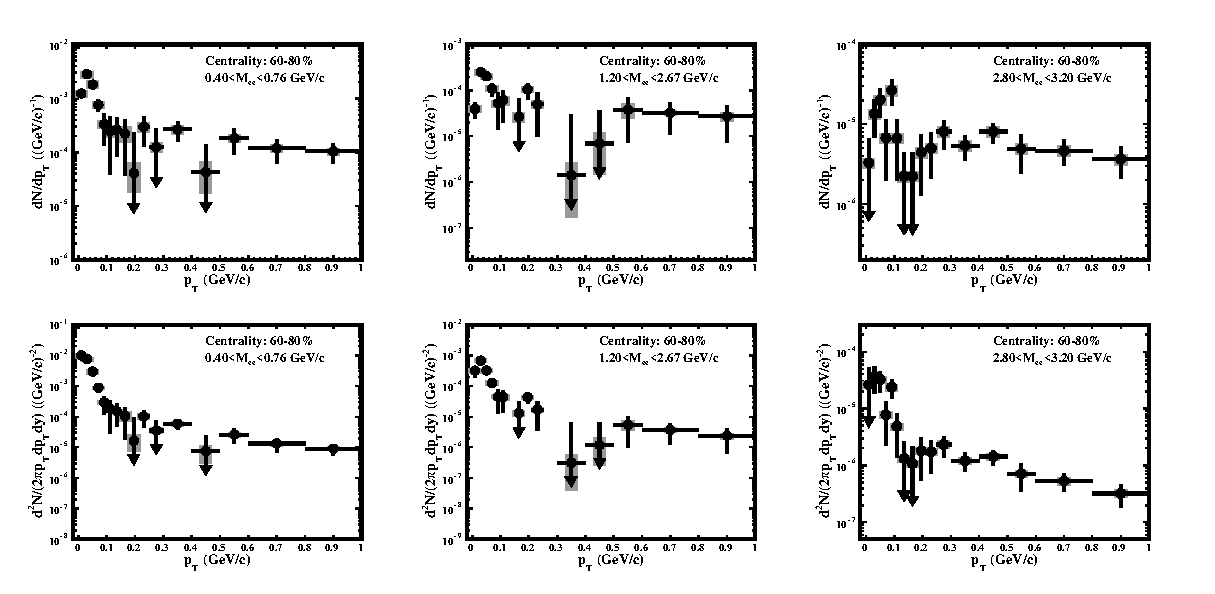
\includegraphics[width=1.0\textwidth]{results/PtSpec_CenBin0.eps}
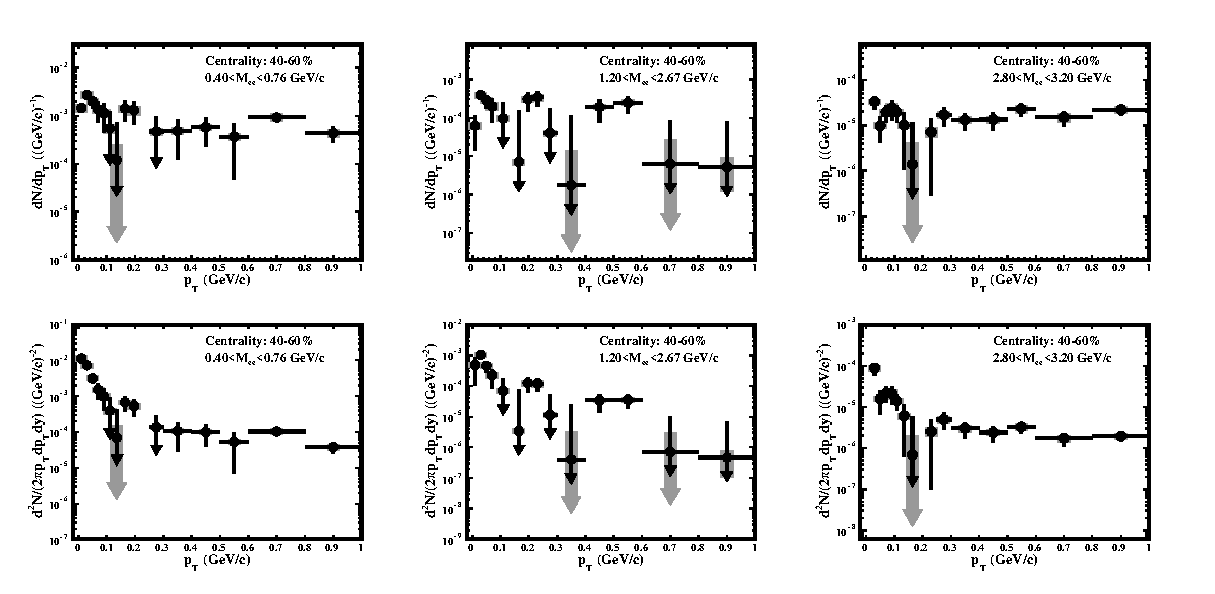
\includegraphics[width=1.0\textwidth]{results/PtSpec_CenBin1.eps}
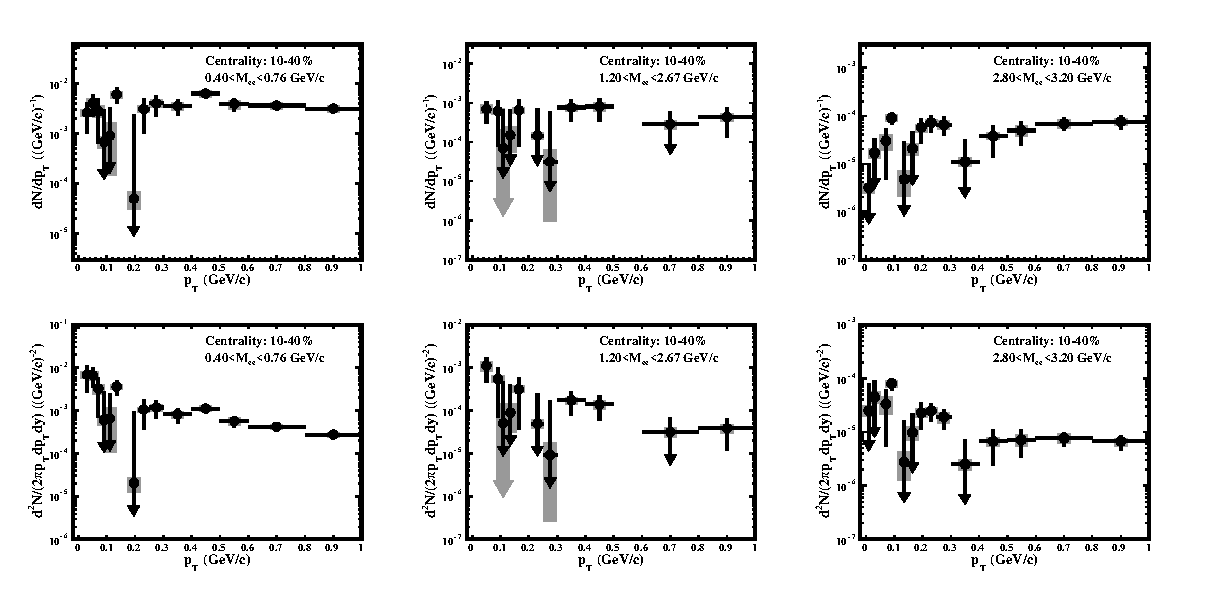
\includegraphics[width=1.0\textwidth]{results/PtSpec_CenBin3.eps}
\figcaption{The efficiency-corrected $dN/dp_{T}$ spectra and cross section as a function of $p_{T}$ within STAR acceptance in  0.40 $<M_{ee}<$ 0.76 GeV/$c^{2}$ (Left column), 1.20 $<M_{ee}<$ 2.67 GeV/$c^{2}$ (Middle column), 2.8 $<M_{ee}<$ 3.2 GeV/$c^{2}$ (Right column) in 60-80\% (Top two rows), 40-60\% (Middle two rows) and 10-40\% (Bottom two rows). Grey boxes (arrows) depict the systematic uncertainties of data.}
\label{ptspec:4diffcens}
\end{figure}
